% !TEX root = DesignDocument.tex

\chapter{User Documentation}

This section contains the end user documentation for the DoorPanes product. It covers the basic setup for using the product and where to go to find the product.

\section{User Guide}

The user guides for the Web Application and Tablet app are included in this section.

\begin{figure}
\centering
  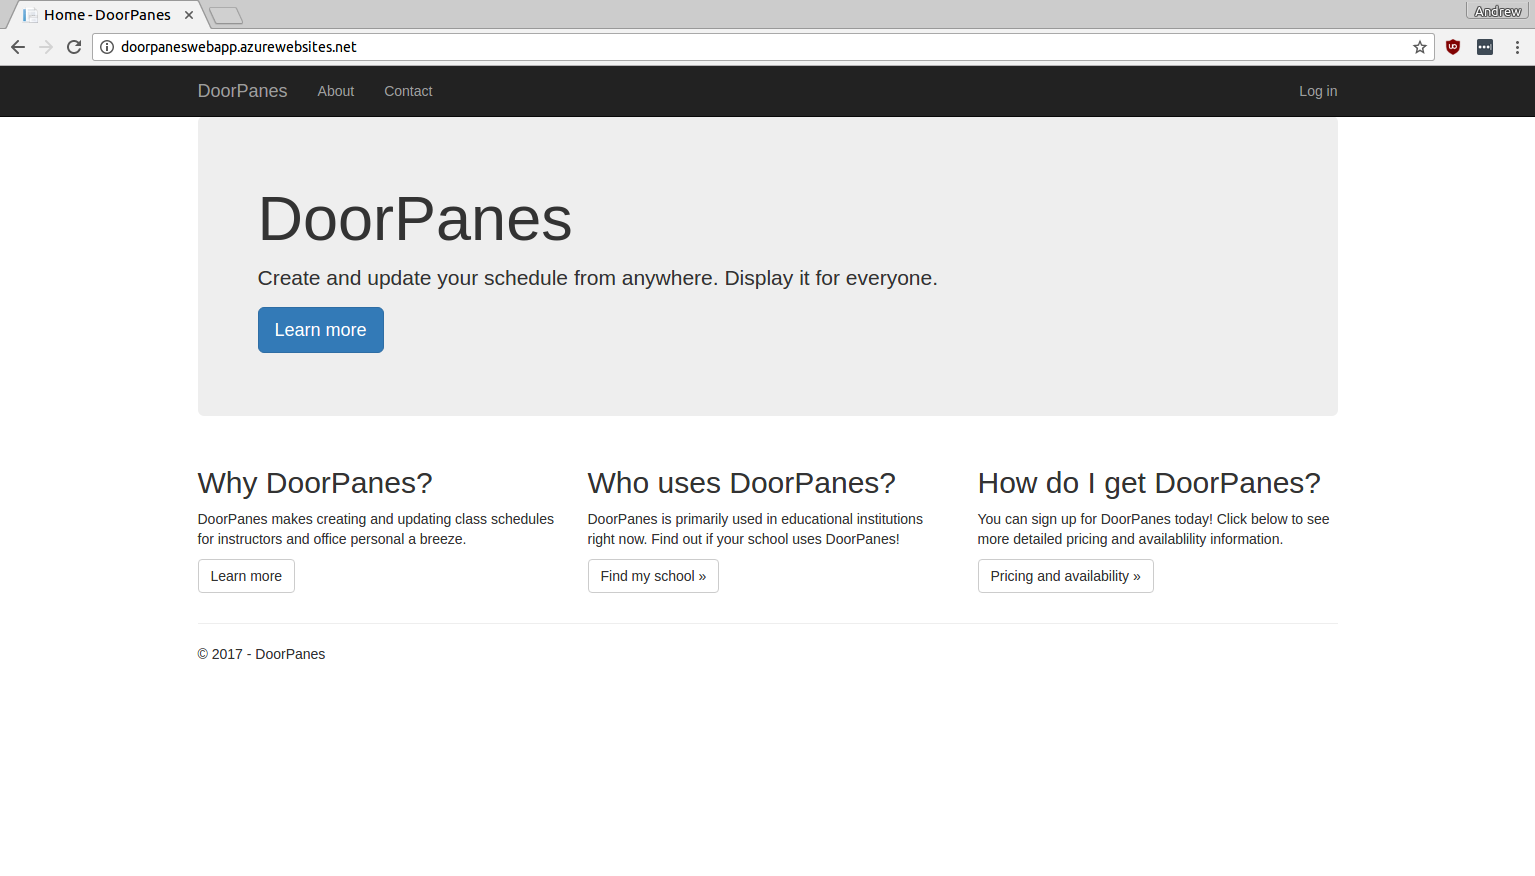
\includegraphics[scale=0.3]{DesignImages/UserGuideImagesWebApp/main_page.png}
  \caption{Main Web Page for Web App}
  \label{fig:main_page}
\end{figure}

\begin{figure}
\centering
  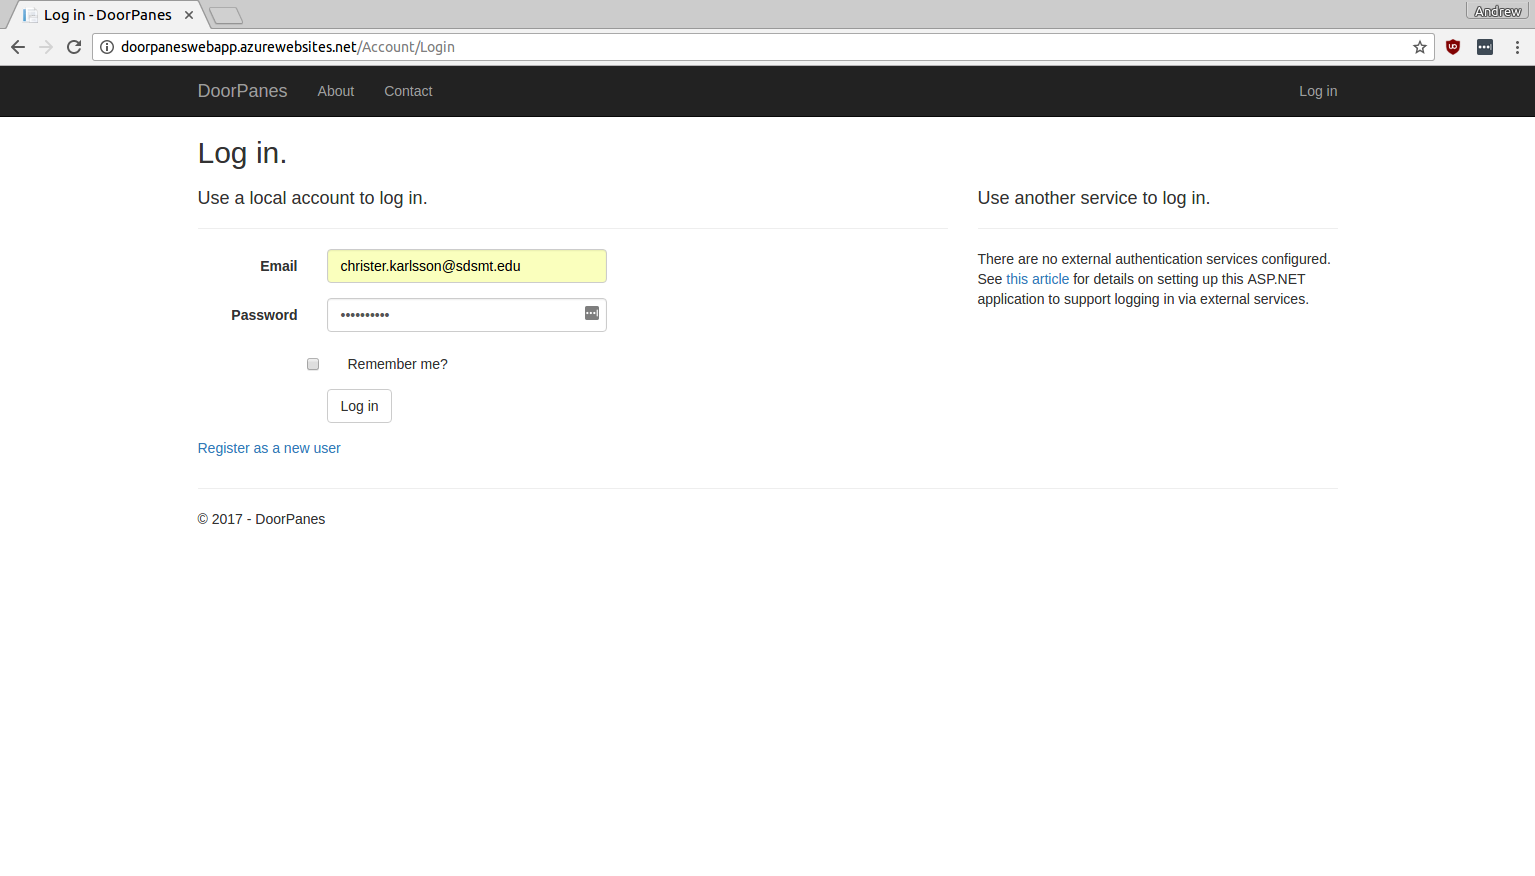
\includegraphics[scale=0.3]{DesignImages/UserGuideImagesWebApp/login_page.png}
  \caption{Main Login Page for Web App}
  \label{fig:login_page}
\end{figure}

\begin{figure}
\centering
  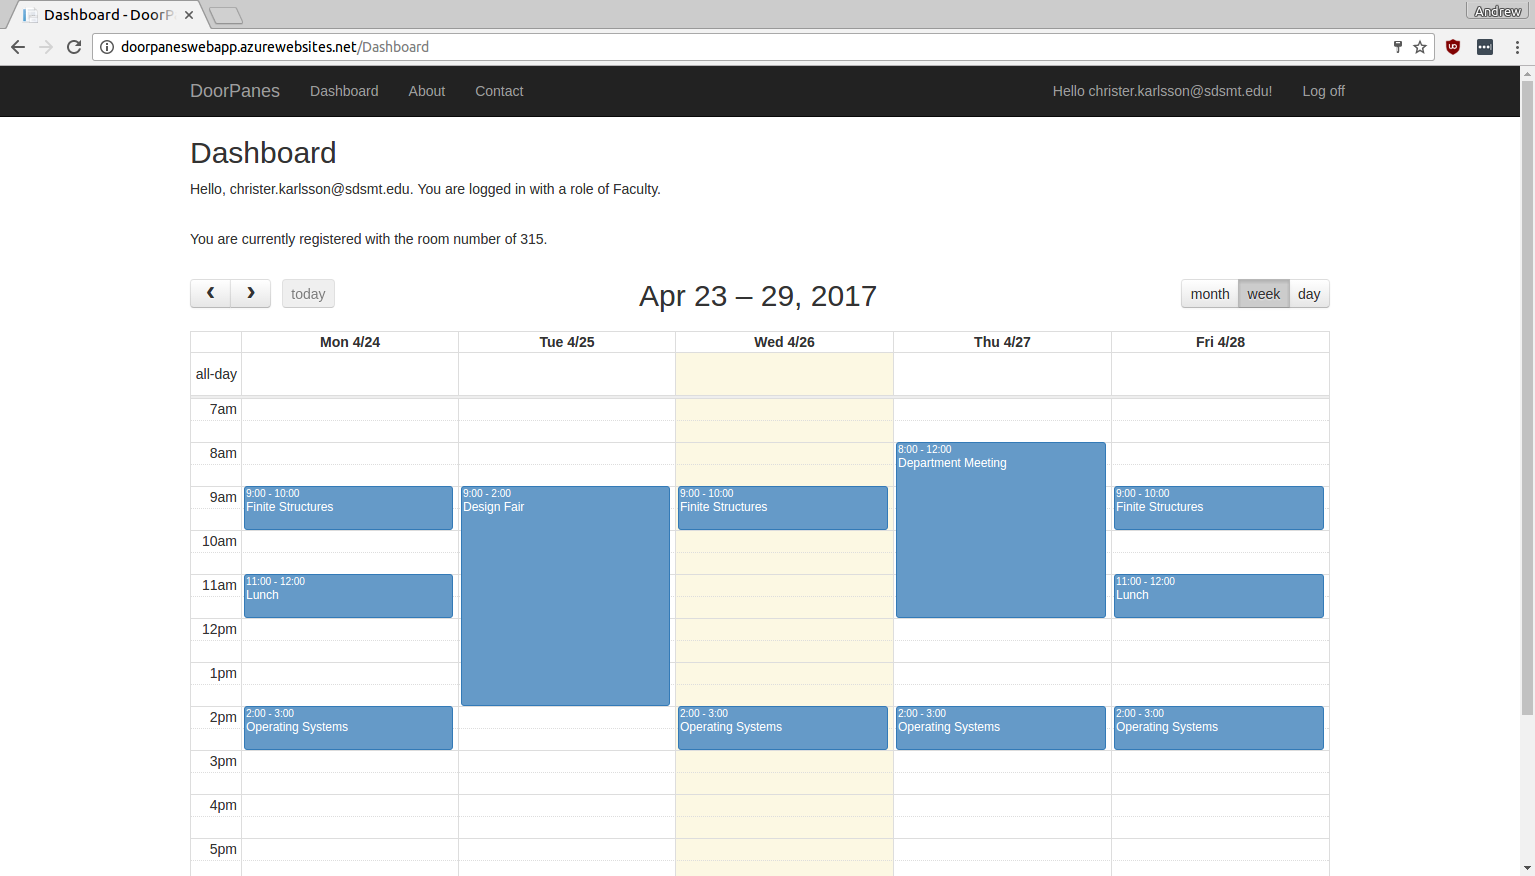
\includegraphics[scale=0.3]{DesignImages/UserGuideImagesWebApp/calendar_view.png}
  \caption{Web App Calendar View}
  \label{fig:calendar_view}
\end{figure}

\begin{figure}
\centering
  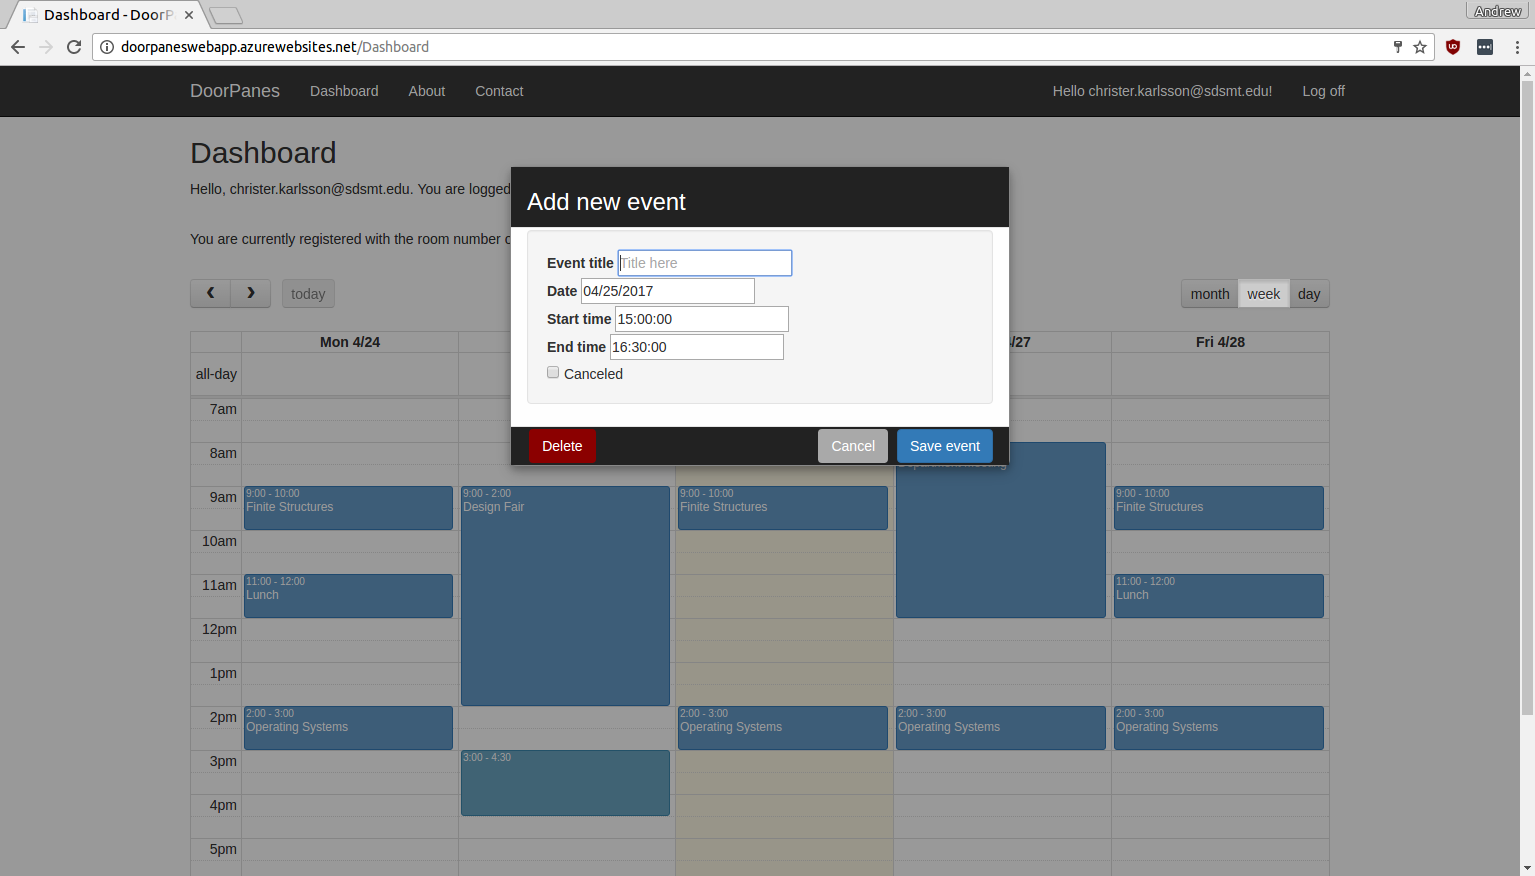
\includegraphics[scale=0.3]{DesignImages/UserGuideImagesWebApp/drag_event.png}
  \caption{Web App Calendar View}
  \label{fig:drag_event}
\end{figure}

\subsection{Web App User Guide} 
% Section Author: Andrew Fagrey
\subsubsection{Navigating to the Web App}
If the web application is live on the web, it can be visited by going to the respective URL. In the case of the development of this project, the URL to go to was www.doorpaneswebapp.azurewebsites.net. Once navigating to the URL in a web browser, the main page will be shown (see the figure below in Figure \ref{fig:main_page}).

Once the Web App is accessible, a user can login to the Web App by clicking the login button in the top left corner, as shown in the figure below (Figure \ref{fig:login_page}).

Once the user has logged in, they will be redirected to the calendar dashboard, where they can add and remove calendar events. This is shown in the figure below (Figure \ref{fig:calendar_view}).


Once a user is viewing the calendar dashboard view, they can add and remove calendar events as they wish. This is shown in Figure \ref{fig:drag_event} .



\subsection{Tablet App User Guide}
Once downloaded, the tablet app will be available for use on Android tablets, preferably using Android 6.0.1.  Details on how to download the app are below.  To use the application, an account must first be made using the web application.  Details about this can be seen above.  

When the app launches, it will ask for log in credentials. Here is where you input your information created on the web application.  The login page can be seen in figure \ref{login} .

\begin{figure}
\centering
  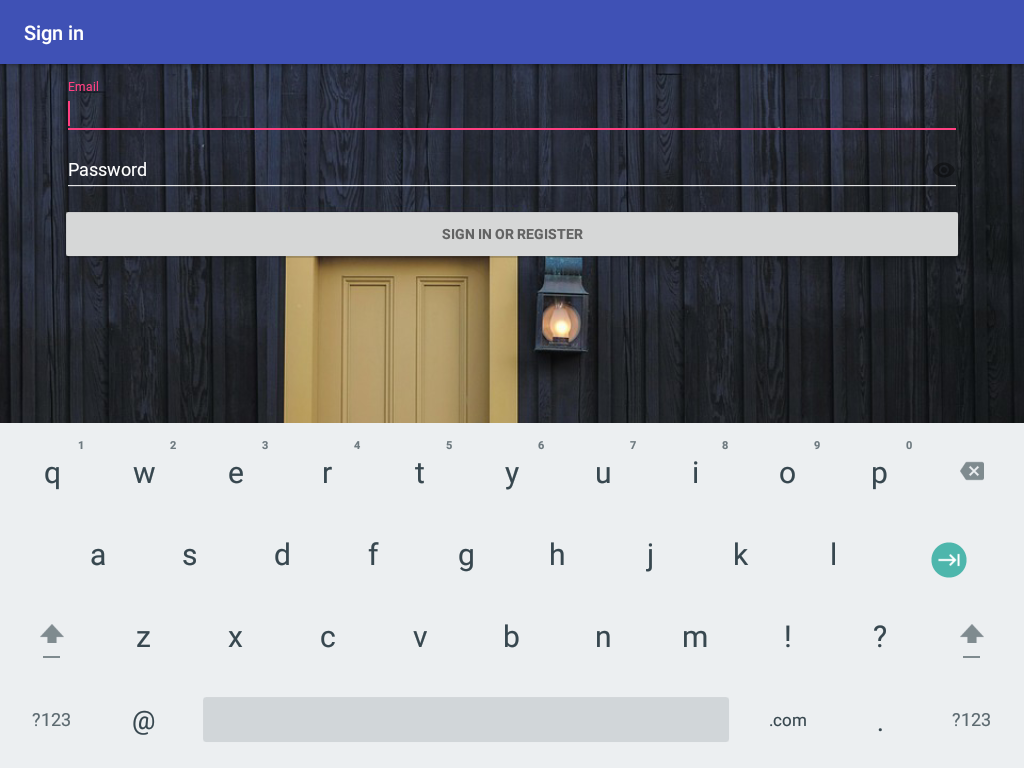
\includegraphics[scale=0.3]{login_final.png}
  \caption{Tablet login page}
  \label{login}
\end{figure}

\begin{figure}
\centering
  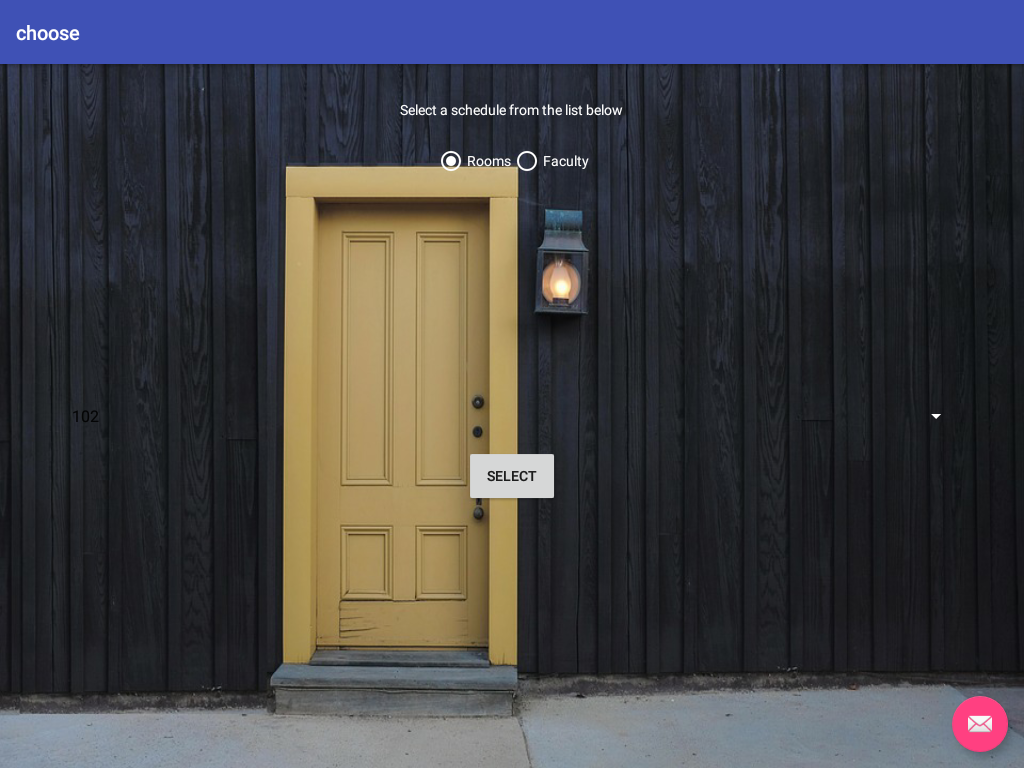
\includegraphics[scale=0.3]{selection_final.png}
  \caption{Tablet calendar selection page}
  \label{selection}
\end{figure}

\begin{figure}
\centering
  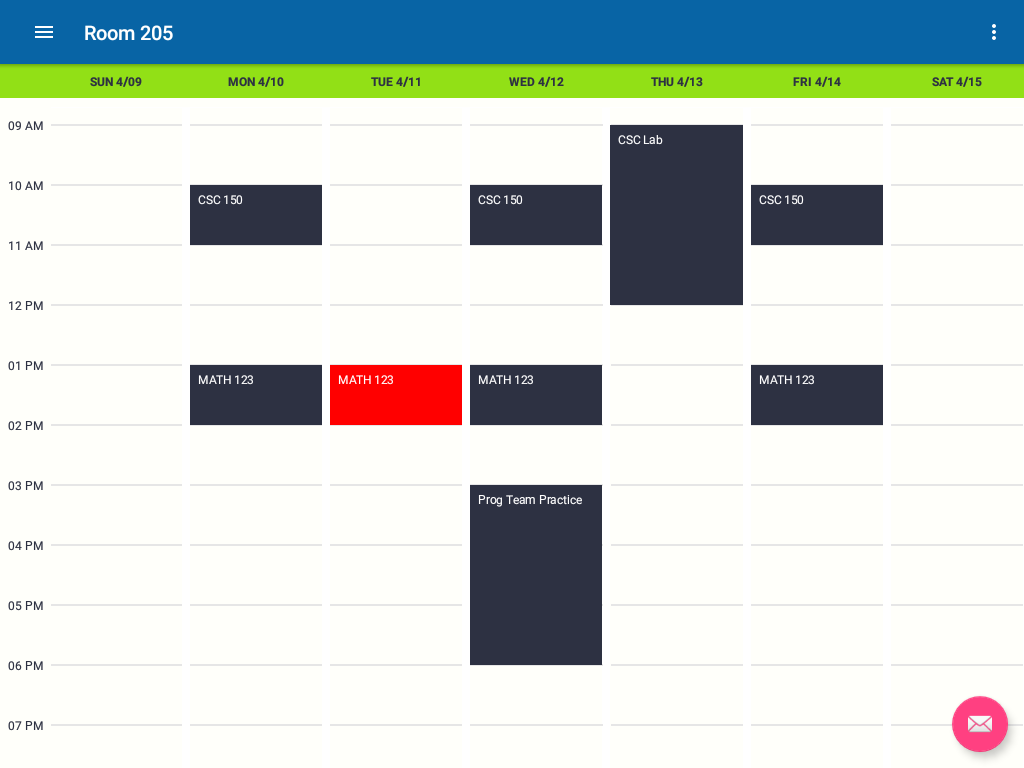
\includegraphics[scale=0.3]{dashboard_final.png}
  \caption{Tablet calendar dashboard}
  \label{dashboard}
\end{figure}

When a user is logged in, Figure \ref{selection} shows the next page that displays a list of available calendars to choose to view.  The radio buttons switch between viewing faculty and room lists.  The dropdown menu shows all the schedules.  Select the schedule you would like to view and press the select button.

When a calendar is selected, the application switches to a different page shown in Figure \ref{dashboard}.  On this page it is important to click the sync button found in the navigation drawer.  Once this button is clicked, the sync process starts and ever 10 seconds a request will be sent to update the events.  Any changes will be updated onto the screen.



On this page all scheduled events will be viewed for that calendar.  To choose a different calendar, simply hit the back button and choose another calendar on the choose page.  








\pagebreak
% Section Author: Andrew Fagrey
\section{Installation Guide}
\subsection{Web App}
The web app is (when uploaded to an Azure service) available as a public website. It can be visited by any computer that has a web browser. There is no need to install any software on your computer to use the web app.

\subsection{Web API}
The web API is not a feature that is available for end users. It is only used by developers to sync data to the tablet app. If you need to use the API, please contact a developer on the project.

\subsection{Tablet App}
The tablet app (once published) would be available from the Google Play store. The process of installing the application would be exactly the same as any other app. A user would visit the Google Play store app on their respective app store and download the app to their tablet that way.
